\section{Model Selection: Optimizing Classifiers for Different Evaluation Metrics}
\begin{multicols}{2}

Now that you've seen a number of different evaluation metrics for both binary and multiclass classification, let's take a look at how you can apply them as criteria for selecting the best classifier for your application, otherwise known as \emph{model selection}. 

In previous lectures we've seen a number of different evaluation frameworks for potential model selection. 

First, we simply did \emph{training and testing on the same dataset}, which as we well know, typically overfits badly and doesn't generalize well to new data. As a side note however, it can serve as a \emph{useful sanity check} to make sure your software engineering and feature generation pipeline is working correctly. 

Second, we frequently use the \emph{train-test split} to produce a single evaluation metric. While fast and easy, this doesn't give as realistic a set of estimates for how well the model may work on future new data. And we don't get a good picture for the variance in the evaluation metrics that may result as we do prediction on different test sets. 

Third, we used \emph{k-fold cross-validation} to create K random train-test splits, where the evaluation metric was averaged across splits. This leads to models that are more reliable on unseen data. 

In particular, we can also use grid search using for example the \texttt{GridSearchCV} method within each cross-validation fold, to find optimal parameters for a model with respect to the evaluation metric.

The default evaluation metric used for a cross-validation score or GridSearchCV is \emph{accuracy}. So how do you apply the new metrics you've learned about here like AUC in model selection? Scikit-learn makes this very easy. You simply add a \texttt{scoring} parameter that's set to the string with the name of the evaluation metric you want to use. 

\subsection{Cross Validation}

Here we're running five folds using a support vector classifier with a linear kernel and C parameter set to one. 

{\scriptsize
\begin{verbatim}
from sklearn.model_selection import cross_val_score
from sklearn.svm import SVC

dataset = load_digits()
# again, making this a binary problem with 'digit 1' 
# as positive class and 'not 1' as negative class
X, y = dataset.data, dataset.target == 1
clf = SVC(kernel='linear', C=1)

# accuracy is the default scoring metric
print('Cross-validation (accuracy)', 
       cross_val_score(clf, X, y, cv=5))
# use AUC as scoring metric
print('Cross-validation (AUC)', 
 cross_val_score(clf, X, y, cv=5, scoring = 'roc_auc'))
# use recall as scoring metric
print('Cross-validation (recall)', 
  cross_val_score(clf, X, y, cv=5, scoring = 'recall'))

Cross-validation (accuracy) 
[0.91944444 0.98611111 0.97214485 0.97493036 0.96935933]
Cross-validation (AUC) 
[0.9641871  0.9976571  0.99372205 0.99699002 0.98675611]
Cross-validation (recall) 
[0.81081081 0.89189189 0.83333333 0.83333333 0.83333333]
\end{verbatim}
}

The first call to cross-val score just uses default \texttt{accuracy} as the evaluation metric. The second call uses the scoring parameter using the string '\texttt{roc_auc}', and this will use AUC as the evaluation metric. The third call sets the scoring parameter to '\texttt{recall}', to use that as the evaluation metric. You can see the resulting list of five evaluation values, one per fold for each metric. 

Now, here we're not doing any parameter tuning we're simply evaluating our model's average performance across multiple folds. 

\subsection{Grid Search}

Now, in this grid search example we use a support vector classifier that uses a \texttt{rbf}~--- radius base function kernel. And the \emph{critical} parameter here is the \texttt{gamma} parameter that intuitively sets the radius or width of influence of the kernel. We use \texttt{GridSearchCV} to find the value of \texttt{gamma} that optimizes a given evaluation metric in two cases. 

{\tiny
\begin{verbatim}
from sklearn.svm import SVC
from sklearn.model_selection import GridSearchCV
from sklearn.metrics import roc_auc_score

dataset = load_digits()
X, y = dataset.data, dataset.target == 1
X_train, X_test, y_train, y_test = train_test_split(X, y, random_state=0)

clf = SVC(kernel='rbf')
grid_values = {'gamma': [0.001, 0.01, 0.05, 0.1, 1, 10, 100]}

# default metric to optimize over grid parameters: accuracy
grid_clf_acc = GridSearchCV(clf, param_grid = grid_values)
grid_clf_acc.fit(X_train, y_train)
y_decision_fn_scores_acc = grid_clf_acc.decision_function(X_test) 

print('Grid best parameter (max. accuracy): ', grid_clf_acc.best_params_)
print('Grid best score (accuracy): ', grid_clf_acc.best_score_)

# alternative metric to optimize over grid parameters: AUC
grid_clf_auc = GridSearchCV(clf, param_grid = grid_values, 
                            scoring = 'roc_auc')
grid_clf_auc.fit(X_train, y_train)
y_decision_fn_scores_auc = grid_clf_auc.decision_function(X_test) 

print('Test set AUC: ', roc_auc_score(y_test, y_decision_fn_scores_auc))
print('Grid best parameter (max. AUC): ', grid_clf_auc.best_params_)
print('Grid best score (AUC): ', grid_clf_auc.best_score_)

Grid best parameter (max. accuracy):  {'gamma': 0.001}
Grid best score (accuracy):  0.9962880475129918

Test set AUC:  0.99982858122393
Grid best parameter (max. AUC):  {'gamma': 0.001}
Grid best score (AUC):  0.9998741278302142
\end{verbatim}
}

In the first case, we just optimize for average accuracy; in the second case we optimize for AUC. In this particular case the optimal value of gamma happens to be the same, point zero-zero-one, for both evaluation metrics. As we'll see later in other cases, the optimal parameter value can be quite different depending on the evaluation metric used to optimize. 

You can see the complete list of names for the evaluation metric supported by the scoring parameter by running the following code that uses the \texttt{scores} variable imported from sklearn metrics. 

{\scriptsize
\begin{verbatim}
from sklearn.metrics.scorer import SCORERS
print(sorted(list(SCORERS.keys())))

['accuracy', 'adjusted_mutual_info_score', 
'adjusted_rand_score', 'average_precision', 
'balanced_accuracy', 'brier_score_loss', 
'completeness_score', 'explained_variance', 'f1', 
'f1_macro', 'f1_micro', 'f1_samples', 'f1_weighted',
'fowlkes_mallows_score', 'homogeneity_score', 
'mutual_info_score', 'neg_log_loss', 
'neg_mean_absolute_error', 'neg_mean_squared_error',
'neg_mean_squared_log_error', 'neg_median_absolute_error', 
'normalized_mutual_info_score', 'precision', 
'precision_macro', 'precision_micro', 'precision_samples',
'precision_weighted', 'r2', 'recall', 'recall_macro', 
'recall_micro', 'recall_samples', 'recall_weighted', 
'roc_auc', 'v_measure_score']
\end{verbatim}
}

You can see metrics for classification such as the string \texttt{'precision_micro'} that represents micro-averaged precision as well as metrics for regression such as the $R^2$ metric for $R^2$ regression loss. 

Let's take a look at a specific example that shows how a classifier's decision boundary changes when it's optimized for different evaluation metrics. This classification problem is based on the same binary digit classifier training and test sets we've been using as an example throughout the notebook. 

\begin{center}
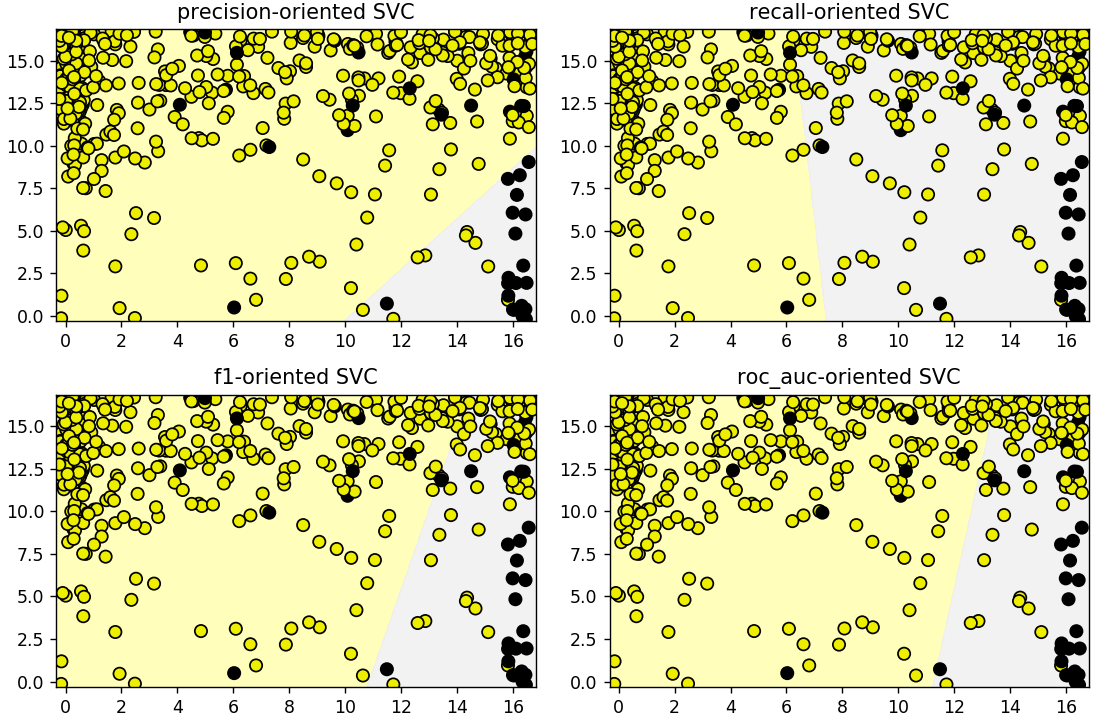
\includegraphics[width=\linewidth]{img/Optimizing-Classifier.png} 
\end{center}


In these classification visualization examples, the positive examples, the digit one are shown as black points and the region of positive class prediction is shown in the light-colored or yellow region to the right of this decision boundary. The negative examples, all other digits, are shown as white points. And the region of negative class prediction here in these figures is to the left of the decision boundary. The data points have been plotted using two out of the 64 future values in the digits' dataset and have been jittered a little. That is, I've added a little bit of random noise so we can see more easily the density of examples in the feature space. 

Here's the scikit-learn code that produced this figure. We apply grid search here to explore different values of the optional class weight parameter that controls how much weight is given to each of the two classes during training. As it turns out, optimizing for different evaluation metrics results in different optimal values of the class weight parameter. As the class weight parameter increases, more emphasis will be given to correctly classifying the positive class instances. 

%\begin{center}
%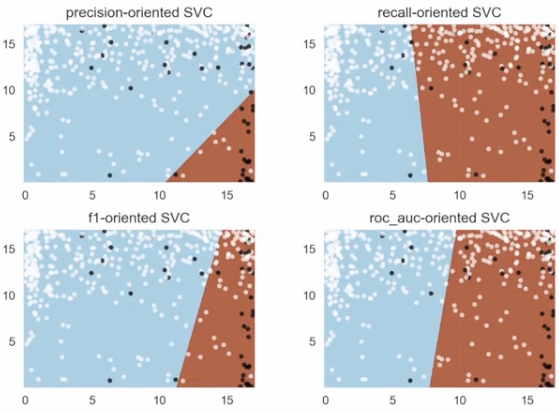
\includegraphics[width=\linewidth]{img/Optimizing-Classifier2.png} 
%\end{center}

The precision-oriented classifier we see here with class weight of two, tries hard to reduce false negatives while increasing true positives. So it focuses on the cluster of positive class points in the lower right corner where there are relatively few negative class points. Here, precision is over 50 percent. 

In contrast, the recall-oriented classifier with class weight of 50, tries hard to reduce the number of false negatives while increasing true positives. That is, it tries to find most of the positive class points as part of its positive class predictions. We can also see that the decision boundary for the F1-oriented classifier has an optimal class weight of two, which is between the optimal class weight values for the precision and recall-oriented classifiers. Visually we can see that the F1-oriented classifier also has a kind of intermediate positioning between the precision and recall-oriented, decision boundaries. This makes sense given that F1 is the harmonic mean of precision and recall. 

The AUC-oriented classifier with optimal class weight to 5 has a similar decision boundary to the F1-oriented classifier, but shifted slightly in favor of higher recall. We can see the precision recall trade-off very clearly for this classification scenario in the precision recall curve for the default support vector classifier with linear kernel optimized for accuracy on the same dataset, and using the balanced option for the class weight parameter. Let's take a look at the code that generated this plot. Take a moment to imagine how the extreme lower right part of the curve on this precision recall curve represents a decision boundary that's highly precision-oriented in the lower right of the classification plot, where there's a cluster of positive examples. 

As the decision threshold is shifted to become less and less conservative, tracing the curve up into the left, the classifier becomes more and more like the recall-oriented support vector classifier example. Again, the red circle represents the precision recall trade-off achieved at the zero score mark, which is the actual decision boundary chosen for the trained classifier. 

For simplicity, we've often used a single train-test split in showing examples of evaluation scoring. However, using only cross-validation or a test set for model selection or parameter tuning may still lead to more subtle forms of overfitting and less optimistic evaluation estimates for future, unseen data. An intuitive explanation for this might be the following: "remember that the whole point of evaluating on a test set is to estimate how well a learning algorithm might perform on future, unseen data. 

The more information we see about our dataset as part of repeated cross-validation passes in choosing our model, the more influence any potential held-up test data has played into selecting the final model. Not merely evaluating it. This is sometimes called data leakage and we'll describe more about that phenomenon in another module. So, we haven't done an evaluation with a truly held-out test set unless we commit to holding back a test split that isn't seen by any process until the very end of the evaluation. 

So that's what's actually done in practice. There are three data splits: training for model building, validation for model selection and a test set for the final evaluation. The training and test sets are typically split out first, and then cross-validation is run using the training data to do model and parameter selection. Again, the test set is not seen until the very end of the evaluation process. Machine learning researchers take this protocol very seriously. The train-validate-test design is a very important universally applied framework for effective evaluation of machine learning models. 

\section{Conclusion}

That brings us to the end of this section of the course on evaluation for machine learning. You should now understand why accuracy only gives a partial picture of a classifier's performance and be more familiar with the motivation and definition of important alternative evaluation methods and metrics of machine learning like confusion matrices, precision, recall, F1 score and area under the RAC curve. 
You've also seen how to apply and choose these different evaluation metric alternatives in order to optimize model selection or parameter tuning for a classifier, to maximize a given evaluation metric. 

Finally, I'd like to leave you with a couple of points. First, simple accuracy may not often be the right goal for your particular machine learning application. As we saw for example with tumor detection or credit card fraud, false positives and false negatives might have very different real-world effects for users or for organization outcomes. So it's important to select an evaluation metric that reflects those user application or business needs. 

Second, there are a number of other dimensions along which it may be important to evaluate your machine learning algorithms, that we don't cover here but that are important for you to be aware of. I'll mention two specifically here. Learning curves are used to assess how a machine learning algorithm's evaluation metric changes or improves as the algorithm gets more training data. Learning curves may be useful as part of a cost-benefit analysis. Gathering training data in the form of labeled examples is often time-consuming and expensive. So being able to estimate the likely performance improvement of your classifier, if you say invest in doubling the amount of training data, can be a useful analysis. Second, sensitivity analysis amounts to looking at how an evaluation metric changes as small adjustments are made to important model parameters. This helps assess how robust the model is to choice of parameters. 

This may be important to perform especially if there are other costs such as runtime efficiency that are critical variables when deploying an operational system, that are correlated with different values of parameter. For example, decision tree depth or future value threshold. In this way, a more complete picture of the trade-offs achievable across different performance dimensions can help you make the best practical deployment decisions for your machine learning model. 

\end{multicols}